% !TEX root = ./../../_Thesis.tex

% section's Name and Label
\subsection{Non-Optical Simulation Techniques}
\label{subsec:NonOpticalSimulationTechniques}

Some techniques are concerned with modeling the effects caused by non-optical issues and use them to achieve more realistic synthetic images. One example is the method proposed by \citet{Deering2005}. His approach describes a retinal photon-accurate model of the human eye. Such a model is used together with computer graphics techniques and a simplified eye's optical model to produce synthetic simulations of the image formation process. 

Another technique that explores different effects caused by the anatomy of the human eye --- the glare --- is discussed by \citet{Ritschel2009}. The authors proposed a model for a real-time dynamic simulation of the scattering in the human eye (Figure~\ref{fig:ritschel_pipeline}), which is efficiently implemented by drawing a few basic primitives, applying an FFT, and doing a special kind of blur. They have also performed psychophysical studies to measure the perception of brightness for glare models. However, they state that, as any other intrinsic phenomena, no ground truth can be obtained. And the model's validation remains a challenging task.

\begin{figure}[h]
	\centering
	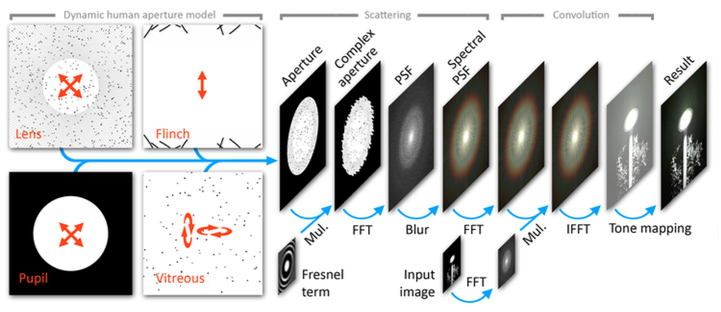
\includegraphics[width=0.99\linewidth]{__Images/03/ritschel_pipeline.png}
	\caption[The temporal glare pipeline]{The temporal glare pipeline \cite{Ritschel2009}.}
	\label{fig:ritschel_pipeline}
\end{figure}